% fig4_algorithm.tex -- the design procedure of Section 4, as a flowchart.
\documentclass[tikz,border=4pt]{standalone}
% ecogstyle.tex -- colours, fonts and plot defaults shared by every figure of
% ecog_coverage.tex.  \input by each standalone figure in this directory.
%
% Colour roles (validated as one categorical palette: adjacent and all-pairs
% CVD separation >= 9, normal-vision separation >= 16; aqua sits below 3:1
% against white, so every aqua mark also carries a marker and a direct label):
%   cBlue    contacts placed by covering radius, single coverage (k = 1)
%   cOrange  the documented 8x8 subdural grid
%   cAqua    contacts restricted to gyral crowns (what a sheet can reach)
%   cViolet  contacts placed by covering radius, double coverage (k = 2)
%   cRed     cortex no contact sees; an onset zone that is missed
\usepackage{amsmath,amssymb}
\usepackage{lmodern}
\usepackage[T1]{fontenc}
\usepackage{tikz}
\usepackage{pgfplots}
\pgfplotsset{compat=1.18}
\usetikzlibrary{arrows.meta,positioning,shapes.geometric,shapes.misc,
  calc,fit,backgrounds,decorations.pathreplacing,patterns,shadows}
\usepgfplotslibrary{fillbetween,groupplots}

\definecolor{cBlue}{HTML}{2A78D6}
\definecolor{cOrange}{HTML}{EB6834}
\definecolor{cAqua}{HTML}{1BAF7A}
\definecolor{cViolet}{HTML}{4A3AA7}
\definecolor{cRed}{HTML}{E34948}
\definecolor{cInk}{HTML}{0B0B0B}
\definecolor{cInk2}{HTML}{52514E}
\definecolor{cMuted}{HTML}{8A8983}
\definecolor{cGrid}{HTML}{E4E3DF}
\definecolor{cSurface}{HTML}{FCFCFB}
\definecolor{cWash}{HTML}{F3F2EF}
\definecolor{cCortex}{HTML}{D9CFC4}
\definecolor{cCortexDark}{HTML}{9C8B7A}
\definecolor{cBlueLight}{HTML}{CDE2FB}
\definecolor{cBlueMid}{HTML}{86B6EF}

\pgfplotsset{
  ecog/.style={
    width=7.2cm, height=5.4cm,
    axis line style={cInk2, line width=0.5pt},
    tick style={cInk2, line width=0.5pt},
    major tick length=3pt,
    grid=major,
    grid style={cGrid, line width=0.4pt, solid},
    tick label style={font=\footnotesize, text=cInk2},
    label style={font=\small, text=cInk},
    title style={font=\small\bfseries, text=cInk, align=center},
    legend style={font=\footnotesize, draw=none, fill=white,
      fill opacity=0.9, text opacity=1, text=cInk,
      row sep=1pt, inner sep=2pt},
    legend cell align=left,
    every axis plot/.append style={line width=1.4pt, line join=round,
      line cap=round},
    axis background/.style={fill=white},
    clip marker paths=true,
  },
  mk/.style={mark=*, mark size=2.1pt,
    mark options={solid, draw=white, line width=0.6pt}},
  mksq/.style={mark=square*, mark size=2.0pt,
    mark options={solid, draw=white, line width=0.6pt}},
  mktri/.style={mark=triangle*, mark size=2.6pt,
    mark options={solid, draw=white, line width=0.6pt}},
  mkdia/.style={mark=diamond*, mark size=2.7pt,
    mark options={solid, draw=white, line width=0.6pt}},
}

% panel letters
\newcommand{\panel}[1]{\textbf{\sffamily (#1)}}
\tikzset{
  panellabel/.style={font=\small\bfseries\sffamily, text=cInk,
    anchor=north west, inner sep=0pt},
  note/.style={font=\footnotesize, text=cInk2, align=center},
}

\begin{document}
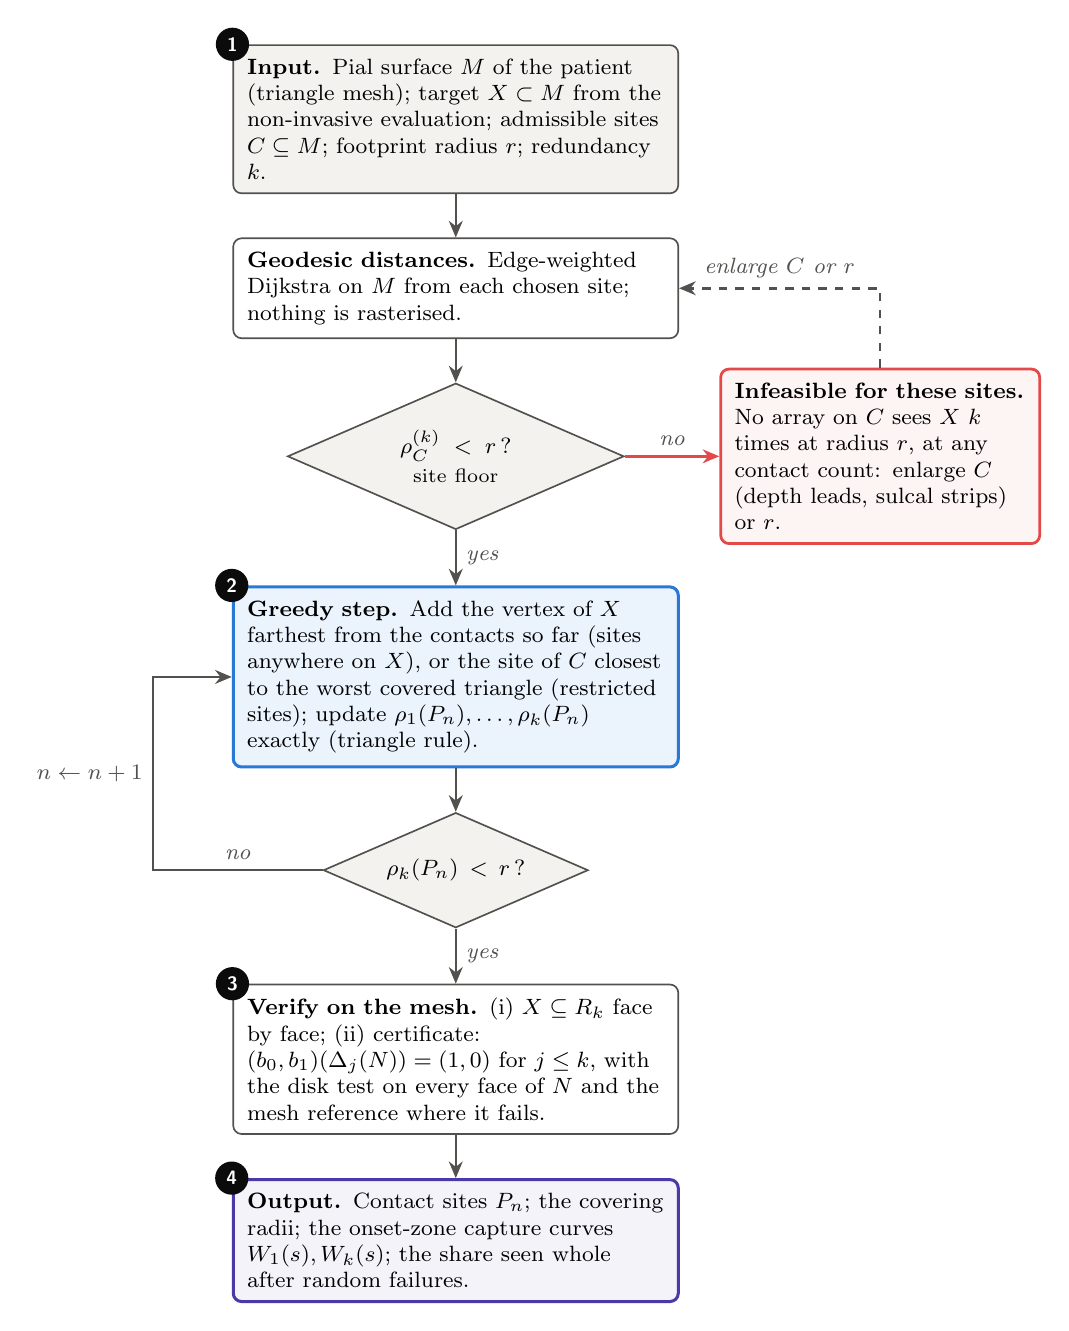
\begin{tikzpicture}[
  font=\footnotesize,
  node distance=0.55cm and 0.9cm,
  proc/.style={rectangle, rounded corners=3pt, draw=cInk2, line width=0.6pt,
    fill=white, align=left, text width=5.3cm, inner sep=5pt,
    execute at begin node=\raggedright},
  io/.style={proc, fill=cWash, draw=cInk2},
  key/.style={proc, draw=cBlue, line width=1.1pt, fill=cBlueLight!40},
  dec/.style={diamond, aspect=2.3, draw=cInk2, line width=0.6pt, fill=cWash,
    align=center, inner sep=0.5pt, text width=2.6cm},
  outbox/.style={proc, draw=cViolet, line width=1.1pt, fill=cViolet!6},
  stop/.style={proc, draw=cRed, line width=1.0pt, fill=cRed!6, text width=3.7cm},
  flow/.style={-{Stealth[length=6pt,width=5pt]}, line width=0.9pt, cInk2},
  lab/.style={font=\footnotesize\itshape, text=cInk2},
  num/.style={circle, fill=cInk, text=white, font=\scriptsize\bfseries\sffamily,
    inner sep=1pt, minimum size=12pt},
]
\node[io] (in) {\textbf{Input.} Pial surface $M$ of the patient (triangle mesh);
  target $X\subset M$ from the non-invasive evaluation; admissible sites
  $C\subseteq M$; footprint radius $r$; redundancy $k$.};
\node[proc, below=of in] (dist) {\textbf{Geodesic distances.} Edge-weighted
  Dijkstra on $M$ from each chosen site; nothing is rasterised.};
\node[dec, below=of dist] (floor) {$\rho_C^{(k)}<r$\,?\\[1pt]{\scriptsize site floor}};
\node[key, below=0.7cm of floor] (greedy) {\textbf{Greedy step.} Add the vertex
  of $X$ farthest from the contacts so far (sites anywhere on $X$), or the site
  of $C$ closest to the worst covered triangle (restricted sites); update
  $\rho_1(P_n),\dots,\rho_k(P_n)$ exactly (triangle rule).};
\node[dec, below=of greedy] (cover) {$\rho_k(P_n)<r$\,?};
\node[proc, below=0.7cm of cover] (verify) {\textbf{Verify on the mesh.}
  (i) $X\subseteq R_k$ face by face;
  (ii) certificate: $(b_0,b_1)(\Delta_j(N))=(1,0)$ for $j\le k$, with the
  disk test on every face of $N$ and the mesh reference where it fails.};
\node[outbox, below=of verify] (outp) {\textbf{Output.} Contact sites $P_n$; the
  covering radii; the onset-zone capture curves $W_1(s),W_k(s)$; the share
  seen whole after random failures.};
% side branches
\node[stop, right=1.2cm of floor] (nofloor) {\textbf{Infeasible for these sites.}
  No array on $C$ sees $X$ $k$ times at radius $r$, at any contact count:
  enlarge $C$ (depth leads, sulcal strips) or $r$.};
\coordinate (loop) at ($(greedy.west)+(-1.0,0)$);
% arrows
\draw[flow] (in) -- (dist);
\draw[flow] (dist) -- (floor);
\draw[flow] (floor) -- node[lab, right] {yes} (greedy);
\draw[flow, cRed] (floor) -- node[lab, above] {no} (nofloor);
\draw[flow] (greedy) -- (cover);
\draw[flow] (cover) -- node[lab, right] {yes} (verify);
\draw[flow] (cover.west) -| node[lab, pos=0.25, above] {no}
  node[lab, pos=0.75, left, font=\footnotesize] {$n\leftarrow n+1$} (loop) -- (greedy.west);
\draw[flow] (verify) -- (outp);
\draw[flow, dashed, cInk2] (nofloor.north) |- node[lab, pos=0.75, above] {enlarge $C$ or $r$}
  (dist.east);
% step numbers
\node[num] at (in.north west) {1};
\node[num] at (greedy.north west) {2};
\node[num] at (verify.north west) {3};
\node[num] at (outp.north west) {4};
\end{tikzpicture}
\end{document}
